\documentclass[a4paper,10pt]{article}

%------------------FORMATTAZIONE E LAYOUT + LINGUA (per evitare errori con hyperref)
\usepackage[T1]{fontenc}
\usepackage[utf8]{inputenx}
\usepackage[english,italian]{babel}
\usepackage{lmodern}
%\usepackage[top=3cm, bottom=3cm, left=2.5cm, right=2.5cm]{geometry}

% Rende il token @ attivo, questo è utile per ri-definire comandi come \aux@chap, nascosti di solito:
\makeatletter

%%%%%%%%%%%%%---DO NOT EDIT---%%%%%%%%%%%%%
%
% standard page settings, 					The new requirements
%* \paperwidth=597.50787pt
%* \paperheight=845.04684pt
%* \textwidth=345.0pt 						%* \textwidth=425.0pt 			
\textwidth=425.0pt
%* \textheight=598.0pt						%* \textheight=635.0pt
\textheight=635.0pt
%* \oddsidemargin=54.0pt					%* \oddsidemargin=0.46pt
\oddsidemargin=0.46pt
%* \evensidemargin=54.0pt				%* \evensidemargin=27.0pt
\evensidemargin=27.0pt
%* \topmargin=17.0pt							%* \topmargin=-10.0pt
\topmargin=-10.0pt
%* \headheight=12.0pt						%* \headheight=13.0pt
\headheight=14.0pt
%* \headsep=25.0pt
%* \topskip=10.0pt
%* \footskip=30.0pt
\footskip=40.0pt
%* \marginparwidth=57.0pt				%* \marginparwidth=57.0pt
\marginparwidth=57.0pt
%* \marginparsep=11.0pt
%* \columnsep=10.0pt
%* \skip\footins=9.0pt plus 4.0pt minus 2.0pt
%* \hoffset=0.0pt
%* \voffset=0.0pt
%* \mag=1000
%* \@twocolumnfalse
%* \@twosidefalse
%* \@mparswitchfalse
%* \@reversemarginfalse
%* (1in=72.27pt=25.4mm, 1cm=28.453pt)
%
%%%%%%%%%%%%%---DO NOT EDIT---%%%%%%%%%%%%%
%

%-------------------------LAYOUT E MODIFICHE
\usepackage{fancyhdr}
\pagestyle{fancy}

% Reset chapter counter at every \c@part increase:
\@addtoreset{chapter}{part}

 % leaving blank the "author" environment:
\author{}

% Command for noun or textsc:
\newcommand{\noun}[1]{\textsc{#1}}

\def\chaptermark#1{%
	\markboth{%
		\ifnum \c@secnumdepth>\m@ne
 			Cap. \thechapter.\ 
 		\fi\MakeUppercase{#1}%
 	}{}%
}

 

\usepackage[unicode=true,
 hypertexnames=false,
 bookmarks=true,
 bookmarksnumbered=true,
 bookmarksopen=false,
 breaklinks=false,
 pdfborder={0 0 1},
 backref=false, 
 colorlinks=true%
]{hyperref}
\hypersetup{pdftitle={Spettroscopia vibrazionale},
 pdfauthor={Andrea Maiani},
 linkcolor=blue, 
 citecolor=green,
 urlcolor=cyan, 
 filecolor=red, 
 pdfpagelayout=OneColumn, 
 pdfnewwindow=true, 
 pdfstartview=XYZ, 
 plainpages=false%
}

%-------------------------GRAFICA
% \usepackage{graphicx}
% \usepackage{caption}
% \usepackage{subcaption}
% \usepackage{float}
% \usepackage{wrapfig}
\usepackage{booktabs}
% \usepackage{multirow}

%\usepackage{color}
% \usepackage[dvipsnames]{xcolor}

\usepackage{todonotes}
%-----------------------MATEMATICA-----------------------
\usepackage{amsmath,amssymb,amsthm}
\usepackage{fixmath}

\newtheorem{thm}{Teorema}[section]
\newtheorem{df}{Definizione}[section]
\newtheorem{lem}{Lemma}[section]
\newtheorem{post}{Postulato}[section]

\usepackage{physics}
\usepackage{siunitx}
\sisetup{locale = FR}


\newcommand*{\uuline}[1]{\underline{\underline{#1}}}

\usepackage[version=4]{mhchem} 
% \usepackage{listings}

% Make numbering in the enumerate environment by letter rather than number
\renewcommand{\labelenumi}{\alph{enumi}.}
\numberwithin{equation}{section}

\begin{document}
\title{\vspace{-2cm}Spettroscopia vibrazionale}
\author{\noun{Andrea Maiani}}
\date{\today}
\maketitle

\section{Legge di Lamber-Beer}

La legge di Lambert-Beer è una legge empirica che lega l'intensità della radiazione man mano che essa si propaga all'interno di un mezzo assorbente. Partendo dall'ipotesi, giustificata da evidenze sperimentali, che la diminuzione percentuale dellì'intensità della radiazione è proporzionale alla concentrazione del soluto $c$ e della lungezza della cella di analisi $\dd x$, ossia in formule:

\begin{equation}
- \frac{\dd I}{I} = \epsilon c \dd x 
\end{equation}

dove la costante di proporzionalità $\epsilon$ è il coefficiente di estinzione molare. Integrando l'equazione tramite separazione di variabili si arriva al risultato:

\begin{equation}
I=I_0 e^{-c \epsilon L}
\end{equation}

Questo risultato è importante poiché la capacità di assorbimento $\epsilon$ della misciela è funzione della frequenza della radiazione $\nu$ e dunque sarà legato alla probabilità di transizione per unità di tempo nella descrizione quantomeccanica. Altri parametri che influiscono sull'assorbanza sono rappresentati dipendenza dalle condizioni di esercizio: temperatura se liquido, pressione e temperatura in un gas.

\section{Spettroscopia infrarossa}

L'interazione di una molecola con la radiazione infrarossa, ossia la porzione di spettro elettromagnetico nel quale l'energia del fotone è comparabile con quella dei gap energetici tra gli stati vibrazionali, è ben descritta tramite la teoria delle perturbazioni. Sia dunque $\hat{H}_0$ l'hamiltoniana della molecola indisturbata e $\hat{H}'$ l'hamiltoniana di interazione:

\begin{equation}
\hat{H} = \hat{H_0} + \hat{H}'
\end{equation}

L'hamiltoniana d'interazione $\hat{H}'$ sarà quindi:
\begin{equation}
\hat{H}' = - \vb{E}\cdot\hat{\vb{M}} = -\vb{E}\cdot\left(\sum_\alpha e Z_\alpha \hat{\vb{R}}_\alpha - \sum_i e \hat{\vb{r}}_i \right)
\end{equation}

Studiamo ora il caso dell'interazione con un'onda piana sinusoidale, ossia: $\vb{E}=\vb{E}_0 \cos(\omega t + \phi)$.

\par
La teoria delle piccole perturbazioni dipendenti dal tempo sviluppata al primo ordine ha come risultato finale la regola d'oro di Fermi che permette di calcolare la probabilità di transizione per unità di tempo $\Gamma_{if}$. Per una perturbazione sinusoidale la regola d'oro assune ka forma:
\begin{equation}
\Gamma_{if} = \frac{2\pi}{\hbar} \abs{\bra{f}\hat{H}'\ket{i}}^2 \delta(E_f-E_i-\hbar\omega)
\end{equation}

Dunque sappiamo che non necessario studiare tutto il problema quantistico ma è sufficiente ridursi a studiare gli elementi di matrice dell'hamiltoniana di interazione $\hat{H}'$ che in questo caso, a meno di fattori moltiplicativi, è semplicemente l'operatore momento di dipolo $\hat{\vb{M}}$. Definiamo dunque gli elementi di matrice:
\begin{equation}
\vb{m}_{fi} = \int_V \Psi^*_f \hat{\vb{M}} \Psi_i \dd V
\end{equation}

Proseguiamo sfruttando l'approssimazione di Bohr-Oppenheimer e separiamo l'integrale sui due spazi disgiunti:
\begin{align}
\Psi_i \stackrel{BO}{\simeq} \psi_g \Phi_i && \Psi_f \stackrel{BO}{\simeq} \psi_g \Phi_f
\end{align}

\begin{equation}
\vb{m}_{fi} = \int_{V_n} \Phi^*_f \left( \int_{V_e} \psi^*_g \hat{\vb{M}} \psi_g \dd V_e \right) \Phi_i \dd V_n 
\end{equation}

Rinominiamo l'integrale interno, quest'ultimo è ancora un operatore perchè non è stato integrato su tutto lo spazio delle configurazioni ma solo sul sottospazio elettronico, inoltre il risultato di questa integrazione incompleta dipende dalla autofunzione elettronica dello stato fondamentale che, a causa dell'approssimazione di Born-Oppenheimer, dipende a sua volta dalle coordinate dei nuclei:
\begin{equation}
\hat{\vb{M}}_g (\vb{R}_\alpha) = \int_{V_e} \psi^*_g \hat{\vb{M}} \psi_g \dd V_e
\end{equation}

Abbiamo ricondotto il problema allo spazio vibrazionale della molecola scegliamo dunque di adottare l'approssimazione armonica e passiamo alle coordinate normali poiché, come sappiamo, sfruttando questa base l'autofunzione del sistema vibrazionale è il prodotto di oscillatori armonici semplici:

\begin{equation}
\Phi(\vb{R}_\alpha) = \Phi({Q_k})
\end{equation}

Per semplificare ulteriormente il problema sviluppiamo in serie di Taylor al primo ordine l'operatore $\hat{\vb{M}}_g$, questa operazione è chiamata \textit{approssimazione armonica elettrica}:
\begin{equation}
\hat{\vb{M}}_g \simeq \vb{M}_{g,0} + \sum_k \pdv{\vb{M}_g}{Q_k}\eval_0 \hat{Q}_k 
\end{equation}

\subsection{Analisi monomodale}
Nel caso monomodale siamo di fronte a una molecola che ammette una sola frequenza di risonanza, quindi l'unica transizione possibile sarà quella tra due autostati dell'oscillatore armonico che avranno numeri quantici $v$ e $w$
\begin{align}
\vb{m}_{vw} &= \int_{-\infty}^{+\infty} \Phi^*_w \hat{\vb{M}}_g \Phi_v \dd Q = \\
            &= \int_{-\infty}^{+\infty} \Phi^*_w \vb{M}_{g,0} \Phi_v \dd Q + \int_{-\infty}^{+\infty} \Phi^*_w \pdv{\vb{M}_g}{Q} \eval_0 \hat{Q} \Phi_v \dd Q = \\
            &= \vb{M}_{g,0} \delta_{vw} + \pdv{\vb{M}_g}{\vb{Q}}\eval_0 \bra{w}\hat{\vb{Q}}  \ket{v}
\end{align}

Da questa espressione per l'elemento di matrice dell'operatore momento di dipolo elettrico possiamo dedurre le regole di selezione per l'assorbimento infrarosso di una molecola, infatti quando questo è nullo non è possibile nessuna transizione. 
Il primo termine è nullo se non per $w=v$ quindi rappresenta il momento di dipolo elettrico della molecola nello stato di ground vibrazionale. Il secondo termine invece, per le proprietà degli autostati dell'oscillatore armonico, è nullo se non quando $w$ ed $v$ differiscono di un unità. Da questo deduciamo che la regola di selezione per le transizioni vibrazionali impone che queste avvengano sempre solo tra due autostati adiacenti.

\par
Eseguendo il calcolo esplicito dell'integrale si ottiene la formula generale per l'elemento di matrice:
\begin{equation}
\vb{m}_{wv} = \vb{M}_{g,0} \delta_{vw} + \pdv{\vb{M}_g}{Q}\eval_0  K \delta_{w,v+1}
\end{equation}

Dove $K$ è una costante che vale a seconda che la transizione sia di eccitamento o diseccitamento:
\begin{align} 
K^{+}=\sqrt{\frac{v+1}{2} \frac{\hbar}{\omega}} && K^{-}=\sqrt{\frac{v}{2} \frac{\hbar}{\omega}} \\
\end{align}

La regola di selezione appena descritta però, non assicura che tutte le transizioni descritte avvengano poiché un'altra condizione necessaria è rappresentata dal termine $\pdv{\vb{M}_g}{Q}\eval_0$ che non deve essere nullo. Il significato fisico di questa condizione consiste nella richiesta che l'oscillazione meccanica in questione causi a sua volta un'oscillazione del momento di dipolo. Ad esempio il valore atteso del momento di dipolo non varia lungo il modo totalsimmetrico di una molecola con centro di inversione e dunque la radiazione infrarossa non causa transizioni che eccitino questo modo normale.

\par
In questa descrizione di prima approssimazione non possono sono descritti fenomeni di anarmonicità e overtones per i quali è necessario un modello più evoluto che vada oltre le ipotesi semplificatrici di armonicità meccanica ed elettronica.

\subsection{Analisi multimodale}
Gli autostati vibrazionali nell'analisi multimodale saranno il prodotto di autofunzioni dell'oscillatore armonico con numeri quantici rispettivamente $v_j$ e $w_k$ :

\begin{align}
\Phi_{i} = \prod_j \phi_{v_j} (Q_j) &&
\Phi_{f} = \prod_k \phi_{w_k} (Q_k) 
\end{align}

Per quanto riguarda l'operatore $\hat{\vb{M}}$ vale lo stesso discorso della trattazione monomodale:
\begin{equation}
\hat{\vb{M}}_g = \int_{V_e} \psi_g^* \hat{\vb{M}} \psi_g \dd V_e
\end{equation}

\begin{equation}
\hat{\vb{M}}_g \simeq \vb{M}_{g,0} + \sum_m \pdv{\vb{M}_m}{Q_m}\eval_0\hat{Q}_m 
\end{equation}

Calcoliamo ora l'elemento di matrice dell'operatore momento di dipolo:
\begin{equation}
\vb{m}_{fi} = \vb{M}_{g,0} \int \Phi^*_f \Phi_i \dd \vb{Q} +\sum_m \pdv{\vb{M}_g}{Q_m} \eval_0 \int \Phi^*_i \hat{Q_m} \Phi_f \dd \vb{Q}
\end{equation}

\begin{equation}
\vb{m}_{fi} = \vb{M}_{g,0} \int \Phi^*_f \Phi_i \dd \vb{Q} +\sum_m \pdv{\vb{M}_g}{Q_m} \eval_0 \bra{w_m} \hat{Q}_m \ket{v_m} \prod_{k\neq m} \bra{w_k}\ket{v_k}
\end{equation}

\begin{equation}
\vb{m}_{fi} = \vb{M}_{g,0} \prod_j \delta_{w_j, v_j} + \sum_m \pdv{\vb{M}_g}{Q_m} \eval_0 \delta_{w_k, v_k\pm1} \prod_{m} \delta_{w_m, v_m}
\end{equation}

Da questa espressione possiamo dedurre le regole di selezione: il primo termine non contribuisce poiché è nullo ogni volta che abbiamo una transizione il secondo termine invece è non nullo solo per transizioni tra stati adiacenti e solo in un unico oscillatore alla volta. Questo significa che, in una singola interazione, si può eccitare un solo modo normale e solo portandolo allo stato strettamente più energetico.
Anche nell'analisi multimodale una condizione necessaria per avere una transizione è che il termine $\sum_m \pdv{\vb{M}_g}{Q_m} \eval_0$ sia non nullo. Questo fa si che le molecole che oscillando conservano il loro momento di dipolo non possano andare incontro ad assorbimento od emissione tramite questo meccanismo (sono invisibili alla spettroscopia infrarossa).

\section{Scattering Raman}
La spettroscopia Raman sfrutta lo scattering anelastico di fotoni in un materiale attraversato da un laser a una frequenza a cui esso è trasparente.

\subsection{Interpretazione classica}
Un modello classico dello scattering Raman può essere ottenuto tramite l'analisi della risposta del momento di dipolo $\vb{M}$ di un materiale con tensore di polarizzabilità $\uuline{\alpha}$ non nulla ad un campo elettrico sinusoidale generico del tipo:
\begin{equation}
\vb{E} = \vb{E}_0 \cos (\omega_L t + \phi_L)
\end{equation}

Dove il momento di dipolo è descritto da un termine a riposo e un termine dipendente dalla polarizzabilità $\uuline{\alpha}$:
\begin{equation}
\vb{M} = \vb{M}_0  + \uuline{\alpha}(\vb{Q}) \vb{E} 
\end{equation}

Si procede trascurando $\vb{M}_0$ e approssimando la polarizzabilità con una serie di Taylor al primo ordine:
\begin{equation}
\vb{M} \simeq \left( \uuline{\alpha_0} +\sum_k\pdv{\uuline{\alpha}}{Q_k} \eval_0 Q_k \right) \vb{E}_0 \cos (\omega_L t + \phi_L)
\end{equation}

\begin{equation}
\vb{M} = \uuline{\alpha_0}  \vb{E}_0 \cos (\omega_L t + \phi_L) + \pdv{\uuline{\alpha}}{Q_0} \eval_0 Q_0 \cos(\omega_v t + \phi_v) \vb{E}_0 \cos (\omega_L t + \phi_L)
\end{equation}
 
Se si trascura la risposta istantana rappresentata dal primo termine in cui compare $\uuline{\alpha}_0$ e si sviluppa con le formule di prostaferesi il prodotto dei termini coseno si giunge infine a:
\begin{equation}
\vb{M} = \frac{1}{2} \pdv{ \uuline{\alpha}}{Q_0} \eval_0 Q_0 \vb{E}_0  \cos[ (\omega_L-\omega_v) t + (\phi_L - \phi_v) ]  +  \frac{1}{2} \pdv{ \uuline{\alpha}}{Q_0} \eval_0 Q_0 \vb{E}_0 \cos[(\omega_L + \omega_v) t + (\phi_L+\phi_v)]
\end{equation}

Il termine coseno con la differenza delle pulsazioni laser e vibrazionale descrive il processo Raman Stokes, il secondo termine ha per argomento la somma delle pulsazioni e descrive il processo Raman anti-Stokes.

\subsection{Descrizione quantistica}
Lo scattering Raman è un fenomeno di diffusione anelastica di fotoni: quando un materiale viene attraversato da una radiazione di frequenza $\nu_L$ questa può essere assorbita se esiste un modo di vibrazione eccitabile con questa frequenza, in caso contrario in prima approssimazione, il fascio laser attraversa indisturbato il campione essendo questo trasparente per la radiazione in questione.
\par
In realtà il sistema può comunque esser eccitato ad uno stato virtuale, ossia uno stato che non fa parte degli autostati del sistema. Non essendo uno stato ``reale'' il sistema ritorna allo stato fondamentale istantaneamente riemettendo la stessa radiazione incidente: questo è lo scattering Rayleigh (elastico). Solo una piccola parte della radiazione incidente subisce scattering elastico, e una porzione ancora più piccola subisce lo scattering anelastico, ossia Raman: se il sistema dallo stato virtuale non decade nello stato fondamentale ma in un autostato eccitato la frequenza emessa sarà minore di quella incidente e dalla differenza tra le frequenze si può risalire alla differenza energetica tra lo stato fondamentale e quello eccitato. Quello appena descritto è lo scattering Raman di tipo Stokes; lo scattering di tipo anti-Stokes, invece, è descrotto da una molecola che passa da uno stato già eccitato a uno virtuale e poi ritorna allo stato fondamentale, emettendo quindi una radiazione più energetica di quella incidente.

Una descrizione quantomeccanica dello scattering Raman è ottenuta da una teoria perturbativa al secondo ordine (il primo descrive l'assorbimento infrarosso), ed è quindi molto complicata dal punto di vista matematico. Il risultato finale del calcolo si puù schematizzare nella seguente formula per l'elemento di matrice dell'operatore polarizzabilità:
\begin{equation}
\alpha^{g}_{fi} = \alpha^{g,0} \bra{\psi_f}\ket{\psi_i} + \sum_k \pdv{\alpha^{g}}{Q_k}\eval_0 \bra{w_k}\hat{Q}_k\ket{v_k} \prod_{j\neq k} \bra{w_j}\ket{v_k} 
\end{equation}


\par
Le regole di selezione per la spettroscopia Raman sono le stesse di quella infrarossa: si può eccitare un solo modo alla volta e solo allo stato strettamente più energetio.
\par
È importante notare come l'effetto Raman non dipenda dalla frequenza della radiazione incidente, purché essa sia sufficientemente alta. Se si varia la frequenza del laser l'unico effetto è una traslazione dello spettro della radiazione di scattering. Per questo motivo nella spettroscopia Raman si considerano solo le differenze di frequenza tra i vari picchi e non le frequenze assolute.

\begin{figure}[hb]
  \centering
  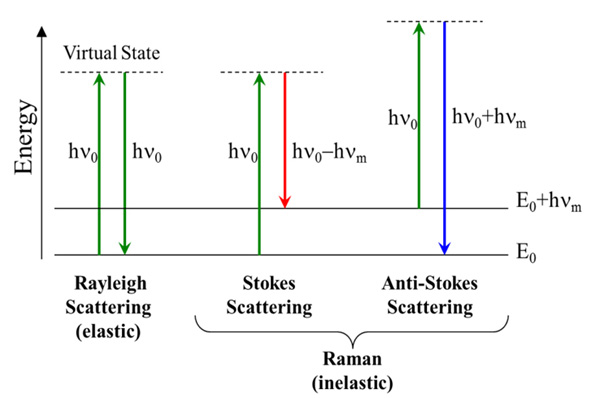
\includegraphics[scale=0.5,keepaspectratio=true]{./raman.jpg}
  % raman.jpg: 0x0 pixel, 300dpi, 0.00x0.00 cm, bb=
  \caption{Scattering elastico ed anelastico}
  \label{fig: raman}
\end{figure}

\section{Altri fenomeni}
\subsubsection*{Alcune frequenze caratteristiche dei legami}
A seguire una breve tabella con alcuni numeri d'onda caratteristici dei legami più comuni. 

\begin{center}
\begin{tabular}{ll}
Legame   & $\tilde{\nu}$ in \si{cm^{-1}}\\
\ce{C-H} & $\sim 3000$\\
\ce{C-D} & $\sim 2000$\\
\ce{C-C} & $\sim 1000$\\
\ce{C=C} & $\sim 1600$\\
\ce{C#C} & $\sim 2100$\\
\end{tabular}
\end{center}

\subsubsection*{Effetto isotopico}
La frequenza normale di vibrazione di un modo dipende dalla massa ridotta, questo significa che isotopi diversi in uno stesso legame hanno frequenze di vibrazioni diverse. Questo comportamento va sotto il nome di \textit{effetto isotopico}.

\subsubsection*{Spettri vibrazionali e simmetria}
Lo spettro vibrazionale di una molecola è intimamente connesso con la sua simmetria: ogni modo normale, infatti, è attivo o meno alla spettroscopia Raman o IR a seconda della specie di simmetria a cui appartiene. Nella tabella dei caratteri le ultime due colonne danno indicazioni sull'attività del modo: se nella penultima colonna compaiono i simboli $x$, $y$, $z$ il modo sarà attivo all'infrarosso; se nell'ultima colonna compaiono monomi di secondo grado il modo sarà attivo all'effetto Raman.

\subsubsection*{Mutua esclusione IR-Raman}
Un altro fenomeno rilevante causato dalla simmetria convolge le molecole il cui gruppo di simmetria contiene un centro di inversione $i$. In questo caso si osserva \textit{mutua esclusione IR-Raman}: se un modo compare nello spettro IR allora non comparirà nello spettro Raman e viceversa. 

\end{document}